\documentclass[12pt,a4paper, openany]{memoir}
% \documentclass[titlepage,12pt,a4paper]{book}

% substituir linha seguinte por 
% \usepackage[english]{babel} 
% se o relatório for escrito na língua inglesa.
\usepackage[portuguese]{babel}

% \usepackage[utf8]{inputenc}
\usepackage[T1]{fontenc}
\usepackage[utf8]{inputenc}

\usepackage{makeidx}
\usepackage{xspace}
\usepackage{graphicx,color,times}
\usepackage{fancyhdr}
% \usepackage{pxfonts}
% \usepackage{times}
% \usepackage{mathptm}
% \usepackage{amssymb}
% \usepackage{amsfonts}

\usepackage{amsmath}
\usepackage{latexsym}
\usepackage[printonlyused]{acronym}
\usepackage{float}
\usepackage{listings}
\usepackage{tocbibind}
\usepackage{natbib}

\usepackage{hyperref}
\hypersetup{
    colorlinks=true,
    linkcolor=blue,
    filecolor=blue,
    urlcolor=blue,
    citecolor=blue,
    %pdftitle={Overleaf Example},
    pdfpagemode=FullScreen,
}

% \usepackage{glossaries}
% \makeglossaries

% \renewcommand{\ttdefault}{phv}


\pagestyle{fancy}
\renewcommand{\chaptermark}[1]{\markboth{#1}{}}
\renewcommand{\sectionmark}[1]{\markright{\thesection\ #1}}
\fancyhf{} \fancyhead[LE,RO]{\bfseries\thepage}
\fancyhead[LO]{\bfseries\rightmark}
\fancyhead[RE]{\bfseries\leftmark}
\renewcommand{\headrulewidth}{0.5pt}
\renewcommand{\footrulewidth}{0pt}
\setlength{\headheight}{14pt}
\setlength{\marginparsep}{0cm}
\setlength{\marginparwidth}{0cm}
\setlength{\marginparpush}{0cm}
\addtolength{\hoffset}{-2cm}
\addtolength{\oddsidemargin}{\evensidemargin}
\addtolength{\oddsidemargin}{0.5cm}
\addtolength{\evensidemargin}{-0.5cm}


\usepackage{fix-cm}
\usepackage{fourier}
\usepackage[scaled=.92]{helvet}
\definecolor{ChapGrey}{rgb}{0.6,0.6,0.6}
\newcommand{\LargeFont}{
  \usefont{\encodingdefault}{\rmdefault}{b}{n}
  \fontsize{60}{80}\selectfont\color{ChapGrey}
  }
\makeatletter
\makechapterstyle{GreyNum}{
  \renewcommand{\chapnamefont}{\large\sffamily\bfseries\itshape}
  \renewcommand{\chapnumfont}{\LargeFont}
  \renewcommand{\chaptitlefont}{\Huge\sffamily\bfseries\itshape}
  \setlength{\beforechapskip}{0pt}
  \setlength{\midchapskip}{40pt}
  \setlength{\afterchapskip}{60pt}
  \renewcommand\chapterheadstart{\vspace*{\beforechapskip}}
  \renewcommand\printchaptername{
  \begin{tabular}{@{}c@{}}
    \chapnamefont \@chapapp\\}
    \renewcommand\chapternamenum{\noalign{\vskip 2ex}}
    \renewcommand\printchapternum{\chapnumfont\thechapter\par}
    \renewcommand\afterchapternum{
  \end{tabular}
  \par\nobreak\vskip\midchapskip}
  \renewcommand\printchapternonum{}
  \renewcommand\printchaptertitle[1]{
  {\chaptitlefont{##1}\par}}
  \renewcommand\afterchaptertitle{\par\nobreak\vskip \afterchapskip}
}
\makeatother
\chapterstyle{GreyNum}

\setcounter{tocdepth}{3}
\setsecnumdepth{subsubsection}

\renewcommand{\ttdefault}{lmtt}


% NEW COLORS
\definecolor{dark}{gray}{0.25}
\definecolor{lgray}{gray}{0.9}
\definecolor{dkblue}{rgb}{0,0.13,0.4}
\definecolor{dkgreen}{rgb}{0,0.6,0}
\definecolor{gray}{rgb}{0.5,0.5,0.5}
\definecolor{mauve}{rgb}{0.58,0,0.82}

\lstset{ %
  language=C,                    basicstyle=\footnotesize,
  numbers=none,                  numberstyle=\tiny\color{gray}, 
  stepnumber=1,                  numbersep=5pt,
  backgroundcolor=\color{white}, showspaces=false,
  showstringspaces=false,        showtabs=false,
  frame=single,                  rulecolor=\color{black},
  tabsize=2,                     captionpos=b,
  breaklines=true,               breakatwhitespace=false,
  title=\lstname,                keywordstyle=\color{blue},
  commentstyle=\color{dkgreen},  stringstyle=\color{mauve},
  escapeinside={\%*}{*)},        morekeywords={*},
  belowskip=0cm
}

\renewcommand{\lstlistingname}{Excerto de Código}
\renewcommand{\lstlistlistingname}{Lista de Excertos de Código}

\renewcommand{\today}{\day \ifcase \month \or Janeiro\or Fevereiro\or Março\or %
Abril\or Maio\or Junho\or Julho\or Agosto\or Setembro\or Outubro\or Novembro\or %
Dezembro\fi de \number \year} 



\begin{document}

\thispagestyle{empty}
\setcounter{page}{-1}

\begin{center}
\begin{Huge}
\textbf{ISCTE}
\end{Huge}
\end{center}

\begin{center}
\begin{Huge}
Iscte School of Technology and Architecture (ISTA)
\end{Huge}
\end{center}

\vspace{0,07cm}
\begin{figure}[!htb]
\centering

\includegraphics[width=200pt]{ISCTE_ISTA.png}
\end{figure}

\vspace{0.5cm}
\begin{center}
\begin{Large}
\textbf{Projeto final de IAA}
\end{Large}
\end{center}


\vspace{0.5cm}
\begin{center}
\begin{normalsize}
\begin{large}
Elaborado por:
\end{large}
\end{normalsize}
\end{center}

\vspace{0.2cm}
\begin{center}
\begin{large}
\textbf{João Filipe Almeida - a127766}

\textbf{Vicente Chã - a127688}
\end{large}
\end{center}

\vspace{0,5cm}
\begin{center}
\begin{normalsize}
\begin{large}
Orientador:
\end{large}
\end{normalsize}
\end{center}

\vspace{0.2cm}
\begin{center}
\begin{large}
\textbf{Professor Doutor Ricardo Ribeiro}
\end{large}
\end{center}



\vspace{0.5cm}
\begin{center}
\begin{normalsize}
\today
\end{normalsize}
\end{center}


\clearpage{\thispagestyle{empty}\cleardoublepage}

\frontmatter

\tableofcontents

\clearpage{\thispagestyle{empty}\cleardoublepage}

\mainmatter
\acresetall
\chapter{\textit{Business Understanding} (João)}
\label{chap:bus}

\section{Definir Objetivos de Negócio}
Na fase inicial do CRISP-DM, o foco esteve em alinhar os objetivos do projeto com as necessidades práticas, o principal objetivo do projeto é prever a probabilidade de ocorrência de doenças cardíacas com base em dados comportamentais e demográficos. O sucesso do projeto será avaliado com base na precisão dos modelos e das suas previsões.

\section{Avaliar a Situação}
Avaliámos os recursos disponíveis, os requisitos, e os potenciais riscos que poderiamos enfrentar:
\begin{itemize}
    \item \textbf{Dados:} Dataset público BRFSS, fornecido pelo \textit{Centers for Disease Control and Prevention (CDC)} \citep{brfss2021}.
    \item \textbf{Requisitos:} Tratar dados, lidar com dados em falta, normalizar, discretizar, reduzir e preparar o dataset para modelos supervisionados e não supervisionados.
    \item \textbf{Riscos:} Possível baixa qualidade, overfitting e eventuais limitações de generalização dos modelos.
\end{itemize}

\section{Plano e estrutura do Projeto}

Desde o inicio que foi planeada e acordada uma estrutura funcional para o projeto onde os modelos pudessem devolver sempre a mesma estrutura de dados que pudesse depois ser alimentada às funções de visualização, criando assim uma distinção entre o a interface e a lógica.
\begin{itemize}
    \item \textbf{Ferramentas:} Uso de \texttt{Python} em junção com Jupyter Notebooks, bibliotecas como \texttt{scikit-learn} e \texttt{pandas}, e \LaTeX para documentação.
    \item \textbf{Etapas por ordem cronológica:}
    \begin{enumerate}
        \item Análise inicial dos dados e exploração.
        \item Preparação dos dados, incluindo tratamento de valores em falta e normalização.
        \item Desenvolvimento dos modelos de previsão.
        \item Comparação e interpretação dos resultados obtidos.
    \end{enumerate}
\end{itemize}

\chapter{\textit{Data Understanding} (Vicente)}
\label{chap2:data_und}

% PERGUNTA 1
\section{O \textit{dataset}}
\label{chap2:dataset}

O \textit{dataset} utilizado para o objetivo do trabalho é composto por 19 categorias, onde cada uma delas tem 308854 atributos dando um total de 5868226 dados para serem trabalhados, sendo a composição de cada categoria a seguinte:

\begin{enumerate}
  \item \textbf{General Health}: Indica a opinião do indivíduo à certa da sua saúde geral, tem como respostas: 'Excellent', 'Fair', 'Good', etc.
  \item \textbf{Checkup}: Indica qual foi a última vez que o individuo foi ao médico, tem como respostas: 'Never', 'Within the past year', etc.
  \item \textbf{Exercise}: Indica se o indivíduo fez algum tipo exercício físico nos ultimos 30 dias, tem como resposta 'Yes' ou 'No'.
  \item \textbf{Heart Disease}: Indica se o individuo tem ou já teve alguma doença coronária ou angina, tem como respostas 'Yes' ou 'No'.
  \item \textbf{Skin Cancer}: Indica se o individuo tem ou já teve cancro da pele, tem com respostas 'Yes' ou 'No'.
  \item \textbf{Other Cancer}: Indica se o individuo tem ou já teve outro tipo de cancro, tem com respostas 'Yes' ou 'No'.
  \item \textbf{Depression}: Indica se o individuo tem ou já teve qualquer tipo transtorno depressivo, tem com respostas 'Yes' ou 'No'.
  \item \textbf{Diabetes}: Indica se o individuo tem ou já teve diabetes, tem como respostas: 'No,' 'No, pre-diabetes or borderline diabetes', 'Yes' e
 'Yes, but female told only during pregnancy'.
  \item \textbf{Arthritis}: Indica se o indivíduo alguma vez foi diagnosticado com artrite, tem com respostas 'Yes' ou 'No'.
  \item \textbf{Sex}: Indica o sexo do indivíduo, tem como respostas 'Female' ou 'Male'.
  \item \textbf{Age Category}: Indica a idade do indivíduo, tem como respostas: '18-24' '25-29' '30-34' ... '80+'.
  \item \textbf{Height (cm)}: Indica a altura do indivíduo sem sapatos em centímetros, tem como respostas: '91.0', '94.0', '96.0', '97.0', '99.0', etc.
  \item \textbf{Weight (kg)}: Indica o peso do indivíduo em sapatos em quilogramas, tem como respostas: '24.95', '25.4', '26.31', '26.76', etc.
  \item \textbf{BMI}: Indica o Índice Massa Corporal do indivíduo, tem como respostas: '12.02', '12.05', '12.11', etc.
  \item \textbf{Smoking History}: Indica se o individuo fuma ou não, tem como respostas 'Yes' ou 'No'.
  \item \textbf{Alcohol Consumption}: Indica quantas vezes o indivíduo bebeu qualquer tipo de bebidas alcoólicas nos últimos 30 dias, tem como respostas: '0', '1', '2', '3', etc.
  \item \textbf{Fruit Consumption}: Indica quantas vezes o indivíduo come fruta, tem como respostas: '0', '1', '2', '3', etc.
  \item \textbf{Green Vegetables Consumption}: Indica quantas vezes  o indivíduo come verduras, tem como respostas: '0', '1', '2', '3', etc.
  \item \textbf{FriedPotato Consumption}: Indica quantas vezes o indivíduo come qualquer tipo de batatas fritas, tem como respostas: '0', '1', '2', '3', etc.
\end{enumerate}

O \textit{dataset} é bem estruturado, com a maioria dos dados claros e de fácil compreensão, no entanto, existem algumas inconsistências que gostaria de apontar.
    
Em relação às categorias 'Alcohol Consumption', 'Fruit Consumption', 'Green Vegetables Consumption' e 'FriedPotato Consumption' (categorias 16, 17, 18 e 19 respetivamente), existe uma inconsistência nos dados adquiridos, as categorias 18 e 19 têm os seus valores entre 0 e 128, a categoria 17 tem os seus valores entre 0 e 120 e a categoria 16 tem os seus valores entre 0 e 30. Isto causa uma grande confusão, pois elas estão todas no mesmo tipo de pergunta, porém devolvem dados diferentes, e isto acontece, pois a pergunta realizada em relação à categoria 16 foi "quantas vezes bebeu álcool nos últimos 30 dias?", e a pergunta realizada para as outras foi "quantas vezes é que come x?". Para ter um \textit{dataset} mais simples e consistente, a questão feita na recolha de dados para as categorias de consumo de comida/bebida deveriam ter sido as mesmas com os mesmos parâmetros de resposta.

As outras inconsistências são menos relevantes que a última e facilmente resolvidas. A categoria 'Age category' apresenta as idades dos indivíduos como pequenos passos entre idades (25 aos 29 anos, 30 aos 34 anos, etc.) mas para a categoria 'Height (cm)' e 'Weight (kg)' isto não acontece, tendo as duas o peso e altura precisa do indivíduo, o que resulta numa quantidade de dados maior que o necessário. Além disso, os valores da categoria 'BMI' apresentam um pequeno desvio do valor real do BMI, e a minha previsão do porquê de isto ocorrer, é porque originalmente o peso e altura eram obtidos em \textit{Feet} e \textit{Inches} e o peso em \textit{pounds} e após a sua conversão para centímetros e quilogramas leva a pequenos desvios no valor original e não foi recalculado o 'BMI'. 

Além destas inconsistências, que serão resolvidas no \ref{chap3:data}, o \textit{dataset} é bem estruturado, todos os seus valores correspondentes à realidade e não existem valores em falta.

Tudo o que foi dito neste capítulo pode ser visualizado gráficamente no código enviado.


% 2. Data Understanding - Vicente

%- 2.1. Collect initial data - ler os dados todos
%- 2.2. Describe data - examinar os dados e descreve-los, as suas propriedades, numero de ocorrencia, etc.
%- 2.3. Explore data - explorar os dados, visualizalos, ver padroes, etc.
%- 2.4. Verify data quality - verificar a integridade dos dados, ver se tem erros, inconsistencias, etc.
\chapter{\textit{Data Preparation}}
\label{chap:data_prep}


% MISSING VALUES
\section{\textit{Missing values} (Ambos)}
\label{chap3:missing_values}

Como foi referido no capítulo \ref{chap2:dataset} o \textit{dataset} não tem valores em falta, por isso tivemos que os criar artificialmente. Para simular valores em falta foi criado um programa que a partir do \textit{dataset} original substituía elementos aleatórios de categorias aleatórias por um valor vazio "None", e a partir daí foram feitos métodos para tentar lidar com estes valores em falta.

\subsection{Método 1 - Substituir pelo valor mais frequente (Vicente)}
\label{chap3:metodo1}

Uma forma comum de lidar com elementos em falta é substituir o valor em falta pelo valor mais frequente na sua categoria especifica, e foi isso que foi implementado neste trabalho. Esta forma foi implementada tal como diz no seu nome, primeiro é calculado e guardado o valor mais frequente de cada categoria, após isso percorremos o \textit{dataset} todo, e se for encontrado um valor em falta, elemento com valor "None", esse elemento é substituído pelo valor mais frequente da categoria a que pertence e a função continua até acabar de percorrer o \textit{dataset}.

\subsection{Método 2 - Fill Missing Values with Mean and Mode (João)}
\label{chap3:metodo2}

Este método lida valores em falta preenchendo-os com a média (em caso de dados numéricos) ou a moda (em caso de dados categóricos) da coluna correspondente.

Este método não remove dados e garante um valor adequado para cada dado em falta de acordo com o seu tipo, sendo um bom compromisso.



% ====================
% DATA NORMALIZATION
% ====================

\section{\textit{Data Normalization}, \textit{Discretization} e \textit{Reduction} (Ambos)}
\label{chap3:data}

\subsection{\textit{Data Normalization} (João)}
\label{chap3:data_norm}

A normalização dos dados é fundamental na preparação algoritmos de aprendizagem automática, especialmente aqueles sensíveis à escala das variáveis como \textit{K-Nearest Neighbors} ou \textit{Multi-Layer Perceptron}.

Foram implementados dois métodos de normalização:

\begin{itemize}
    \item \textbf{\textit{Min-Max Normalization}:} Transforma os valores, trazendo-os para o intervalo \([0, 1]\), segue a seguinte fórmula:
    \[
    x' = \frac{x - x_{min}}{x_{max} - x_{min}}
    \]
    
    onde:
    \begin{itemize}
        \item \( x \) é o valor original.
        \item \( x_{min} \) e \( x_{max} \) são, respetivamente, o menor e o maior valor na coluna.
        \item \( x' \) é o valor normalizado.
    \end{itemize}

    \item \textbf{\textit{Z-Score Normalization}:} Transforma os dados para que tenham uma média de 0 e um desvio padrão de 1. Segue a fórmula:
    \[
    z = \frac{x - \mu}{\sigma}
    \]
    onde:
    \begin{itemize}
        \item \( x \) é o valor original.
        \item \( \mu \) é a média da coluna.
        \item \( \sigma \) é o desvio padrão da coluna.
        \item \( z \) é o valor normalizado.
    \end{itemize}
\end{itemize}

Ambos os métodos foram implementados e podem ser selecionados conforme a necessidade do modelo ou a natureza dos dados.


\subsection{\textit{Data Discretization} (Vicente)}
\label{chap3:data_disc}

Como referido no capítulo \ref{chap2:dataset}, o \textit{dataset} contem inconsistências, e com o uso do \textit{data discretization} é possível removê-las completamente. Para a discriminação dos dados fui ver quais categorias é que tinham o maior número de respostas diferentes, após essa revisão conclui que as categorias 'Height (cm)', 'Weight (kg)', 'BMI','Alcohol Consumption', 'Fruit Consumption', 'Green Vegetables Consumption' e 'FriedPotato Consumption' eram as que mais sofriam de um número exagerado de respostas diferentes.

Para resolver esse problema defini limites para cada uma das categorias e atualizei os seus valores, como, por exemplo, no excerto de código \ref{codigo:data_disc}. A única categoria faço algo mais é o 'BMI', pois como tinha dito no capítulo \ref{chap2:dataset} este tem um pequeno desvio do seu valor real, logo, antes de o categorizar calculo o valor real do BMI através do peso e altura da pessoa, exemplificado na figura \ref{fig:bmi}.


\subsection{\textit{Data Reduction} (Vicente)}
\label{chap3:data_redu}

A redução dos dados foi feita através 3 formas diferentes de redução: eliminação de duplicados, eliminação de categorias inúteis para o objetivo e junção de categorias.

A eliminação de duplicados é bastante óbvia, cada vez que a função de redução é chamada é verificado se o \textit{dataset} tem elementos duplicados, se tiver serão removidos.

De seguida foi feita a remoção das categorias 'General Health' e 'Checkup', pois como o objetivo é tentar prever se um indivíduo tem ou não problemas cardíacos, categorias como as mencionadas não irão influenciar no objetivo. A categoria 'General Health' é uma categoria de opinião sobre a saúde geral do próprio individuo, não tem nenhuma relação com doenças cardíacas. A categoria 'Checkup', apesar da sua temática médica, é apenas uma verificação de quando é que foi a última vez que o individuo foi ao médico, o que não influencia em doenças cardíacas.

O passo principal nesta fase foi a redução das categorias de consumo para uma categoria nova 'qualidade da dieta' (categorias 16, 17, 18 e 19 como referido no capítulo \ref{chap2:dataset}). Para obter criar essa nova categoria decidi calcular o "valor" da dieta de cada indivíduo, para tal somei os valores das categorias 17 e 18 e subtrai as categorias 16 * 4 (a categoria 16 é multiplicada por 4 para dar mais valor no cálculo, pois os seus valores estão só entre 0 e 30) e 19, como indicado no excerto de código \ref{codigo:dieta}. Após isso calculei a média dos valores obtidos e o desvio padrão e defini os parâmetros da nova categoria com eles, após isso verifiquei cada valor de forma semelhante a \ref{codigo:data_disc} e criei a nova categoria como é mostrado na figura \ref{fig:dieta}.

Além destas também pensei em eliminar as categorias 'Height (cm)' e 'Weight (kg)' e deixar apenas o 'BMI', no entanto, achei melhor deixar estar ambas as categorias, pois com o BMI não podemos saber concretamente a altura e peso e apenas com o ele os modelos poderiam obter piores resultados, pois podem existir correlações relevantes entre altura e peso que eu não tenha conhecimento.
\chapter{Modeling}
\label{chap4:modeling}

4. Modeling

- 4.1. Select modeling techniques - os algoritmos que o stor pede no enunciado
- 4.2. Generate test design - dependendo do modelo ter diferentes valores de sets de train, teste e validation
- 4.3. Build model - implementar os modelos
- 4.4. Assess model - interpretar os resultados dos modelos e comprara-los e testalos entre eles para ver qual/quais são os melhores

% SUPERVISED LEARNING
\section{\textit{Supervised Learning} (João)}
\label{chap4:super}

\subsection{\textit{Decision Trees}}
\label{chap4:decision_tree}

Os modelos de \textit{Decision Trees} são amplamente reconhecidos pela sua elevada interpretabilidade, uma vez que o processo de tomada de decisão pode ser visualizado através da árvore gerada. Este método, no entanto, não está livre de \textit{overfitting}, árvores muito complexas podem indicar este fenómeno.

\begin{itemize}
    \item \textbf{Importância das variáveis:} Permite-nos identificar as variáveis mais relevantes para os fins do modelo. A Figura \ref{fig:feature_importance} ilustra as variáveis mais relevantes identificadas.
    \item \textbf{Visualização da árvore de decisão:} A estrutura da árvore, ilustrada na Figura \ref{fig:decision_tree_structure}, demonstra como os dados são particionados em cada nó com base no corte que fornece mais informação. Neste caso, a variável identificada e usada para o nodo raiz foi o `Age\_Category`. 
\end{itemize}

As Figuras \ref{fig:decision_tree_overview}, \ref{fig:feature_importance} e \ref{fig:decision_tree_structure} apresentam respetivamente a matriz de confusão com métricas e tempos, a importância das variáveis e a visualização da estrutura da árvore.


\subsection{\textit{Multi-layer Perceptron}}
\label{chap4:percetrao}

Enquanto as \textit{Decision Trees}, não eram afetadas pela normalização dos dados, no modelo \textit{Multi-layer Perceptron} (MLP) já se verifica uma melhoria significativa dos resultados ao utilizar bases de dados normalizadas

Pode-se verificar na Figura~\ref{fig:mlp_overview} que não está há \textit{overfitting} de nenhuma forma significativo, uma vez que a performance do modelo é parecida quando aplicada de novo ao training set e quando aplicada ao testing set.

Podemos ver também na Figura~\ref{fig:mlp_training_loss} como o erro da \textit{loss function} vai diminuindo ao longo das iterações como é esperado.



\subsection{\textit{k-NN}}
\label{chap4:k-nn}

O modelo de \textit{k-Nearest Neighbors} (k-NN) foi implementado com \(k=3\), ou seja, utilizando os 3 pontos mais próximos para fazer a previsão. Como era esperado, este método exibiu tempos de treino mínimos e tempos de teste mais elevados devido ao cálculo das distâncias. 

Na Figura~\ref{fig:knn_pca} pode-se ver uma distribuição dos dados no espaço reduzido para dimensões pela análise de duas componentes principais para uma representação 2D. Desta forma é possível ter uma ideia de como é que o método funcionará, dá para ver como pontos que representam doença têm tendência a estar juntos e vice versa.








% UNSUPERVISED LEARNING
\section{\textit{Unsupervised Learning} (Vicente)}
\label{chap4:unsuper}

\subsection{\textit{KMeans}}
\label{chap4:kmenas}

O primeiro método de aprendizagem não supervisionada implementado foi o KMeans

\subsection{\textit{DBSCAN}}
\label{chap4:dbscan}
\chapter{Evaluation}
\label{chap:ev}

\section{Avaliar Resultados}
\label{chap:ev:results}

Nesta secção, avaliamos os resultados obtidos para os diferentes modelos, considerando as métricas de desempenho, os tempos de execução e o impacto de diferentes formas de preparação dos dados (original, normalizado, discretizado, etc.).

As quatro métricas principais utilizadas para avaliar os modelos são \textit{accuracy}, \textit{precision}, \textit{recall} e \textit{F1-score}. \textit{Accuracy} mede a proporção de previsões corretas, \textit{precision} avalia a taxa previsões corretas nas previsões positivas e \textit{recall} mede a capacidade de identificar corretamente os casos positivos. O \textit{F1-score} surge como um compromisso que equilibra \textit{precision} e \textit{recall}.

\[
\begin{array}{ll}
\text{Accuracy} & \displaystyle \frac{TP + TN}{TP + TN + FP + FN} \\[2ex]
\text{Precision} & \displaystyle \frac{TP}{TP + FP} \\[2ex]
\text{Recall} & \displaystyle \frac{TP}{TP + FN} \\[2ex]
\text{F1-score} & \displaystyle 2 \cdot \frac{\text{Precision} \cdot \text{Recall}}{\text{Precision} + \text{Recall}}
\end{array}
\]

\noindent Onde:
\begin{itemize}
    \item TP (\textit{True Positives}): Casos positivos corretamente identificados
    \item TN (\textit{True Negatives}): Casos negativos corretamente identificados
    \item FP (\textit{False Positives}): Casos negativos classificados erroneamente como positivos
    \item FN (\textit{False Negatives}): Casos positivos classificados erroneamente como negativos
\end{itemize}


\subsection{Comparação Geral dos Modelos}
A Figura~\ref{fig:model_comparison} apresenta uma representação geral da performance dos modelos. Através daqui pode-se verificar que o modelo com maior taxa de sucesso geral, ou um melhor valor na métrica F1 foi o modelo das Decision Trees.

Nas Figuras \ref{fig:decision_trees_comparison}, \ref{fig:knn_comparison} e \ref{fig:mlp_comparison} conseguimos ver o desempanho dos modelos \textit{Decision Trees}, \textit{Knn} e \textit{Multi Layer Perceptron} respetivamente, quando aplicados a bases de dados tratadas de diferentes formas.

Após uma análise e comparação de todos os métodos, concluímos que o método que nos deu resultados mais desejados, com um F1-Score de 0.217 for o o modelo da \textit{Decision Tree} quando aplicado a uma base de dados Discretizada.

\section{Processo de Revisão}
\label{chap:ev:review}

Uma revisão crítica ao trabalho realizado permite identificar pontos fortes, fracos e áreas de melhoria:
\begin{itemize}
    \item \textbf{Pontos fortes:} A metodologia CRISP-DM garantiu uma abordagem estruturada, fomos capazes de aplicar, treinar, comparar e analisar vários modelos de aprendizagem automática diferentes acabando agora com uma visão mais completa sobre o seu funcionamento num contexto mais prático.
    \item \textbf{Áreas de melhoria:} O baixo desempenho em termos de precisão e recall, e consequentemente no F1-score, pode ser problemático para o diagnóstico de pessoas, especificamente \textit{False Positives} e \textit{True Negatives}
    \item \textbf{Pré-processamento:} Num trabalho futuro podia ser interessante explorar uma base dados não filtrada que nos obrigasse a pensar criticamente sobre valores em falta e como lidar com eles sem termos que ser nós a simular este caso.
\end{itemize}

\section{Próximos Passos}
\label{chap:ev:next_steps}

Com base nos resultados obtidos, consideramos:
\begin{itemize}
    \item \textbf{\textit{Deployment}:} O modelo de \textit{Decision Trees}, devido à sua interpretabilidade e eficiência, é uma escolha adequada para \textit{deployment}. Apesar da \textit{accuracy} ser alta, quando o modelo prevê um "Sim", como é muito mais alto o teor de pessoas que não têm doença, ainda é mais provável que o paciente não tenha do que tenha, causando assim o \textit{Base Rate Neglect}\cite{wikipedia_base_rate_fallacy}. Sedo por isso importante obter uma segunda opinião Médica. 
    \item \textbf{Melhorias potenciais:} Expandir o trabalho para incluir técnicas mais complexas e testar com bases de dados maiores.
\end{itemize}

% \clearpage{\thispagestyle{empty}\cleardoublepage}

\backmatter

\bibliographystyle{plainnat} % Citation style
\bibliography{references}    % Link to the bibliography file (without the .bib extension)

\appendix
\chapter{Imagens}
\label{chap:appendix}

\section{Visualizações específicas}

\begin{figure}[H]
    \centering
    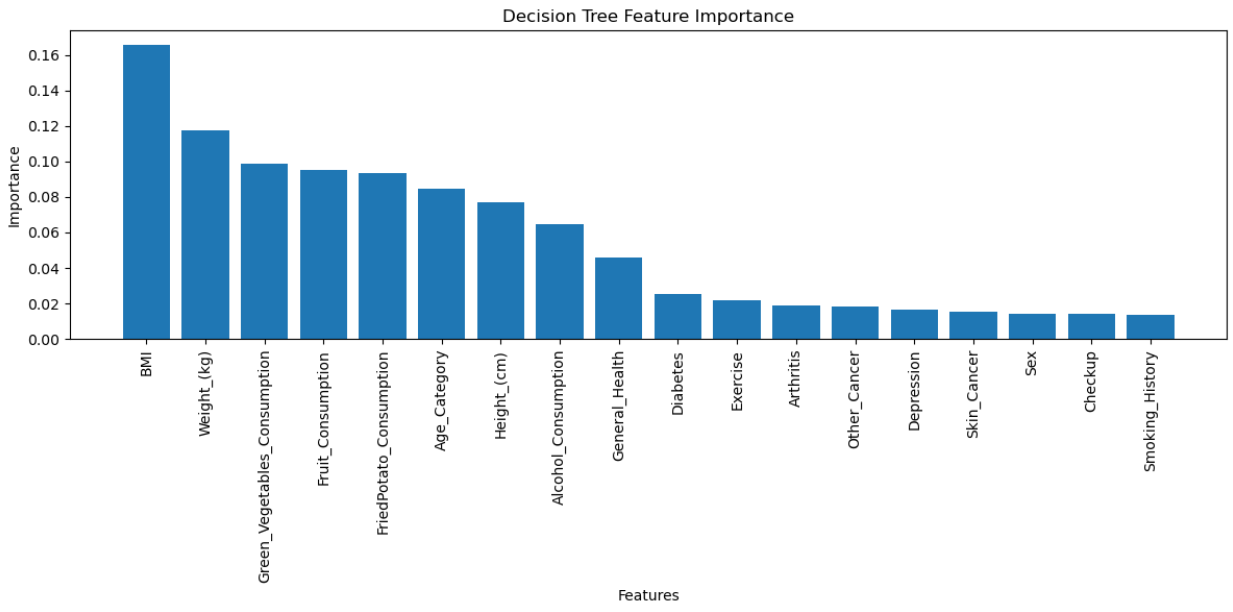
\includegraphics[width=0.9\textwidth]{images/feature_importance.png}
    \caption{\textit{Decision Trees}: Importância das variáveis identificadas pelo modelo.}
    \label{fig:feature_importance}
\end{figure}

\begin{figure}[H]
    \centering
    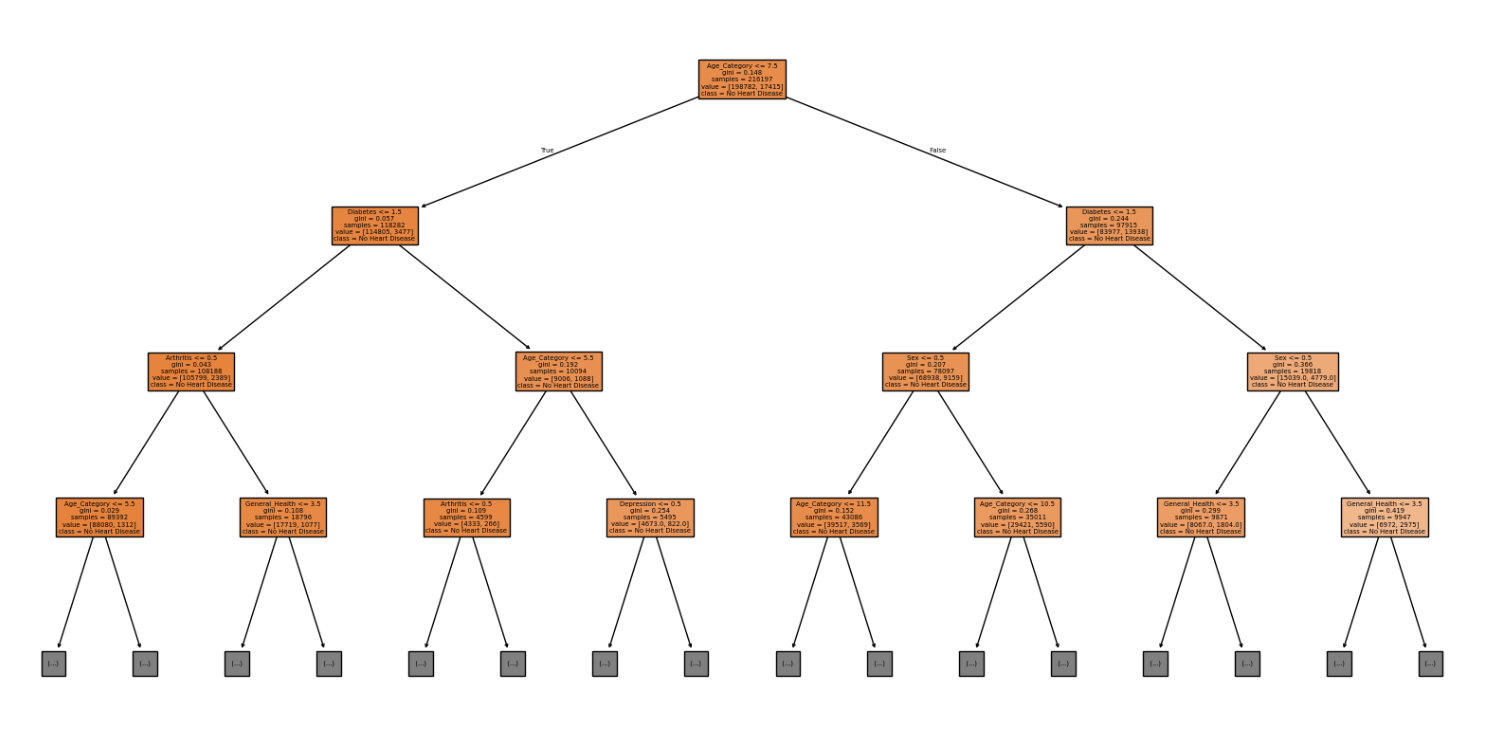
\includegraphics[width=0.9\textwidth]{images/decision_tree_structure.png}
    \caption{\textit{Decision Trees}: Visualização detalhada da estrutura da árvore gerada pelo modelo.}
    \label{fig:decision_tree_structure}
\end{figure}

\begin{figure}[H]
    \centering
    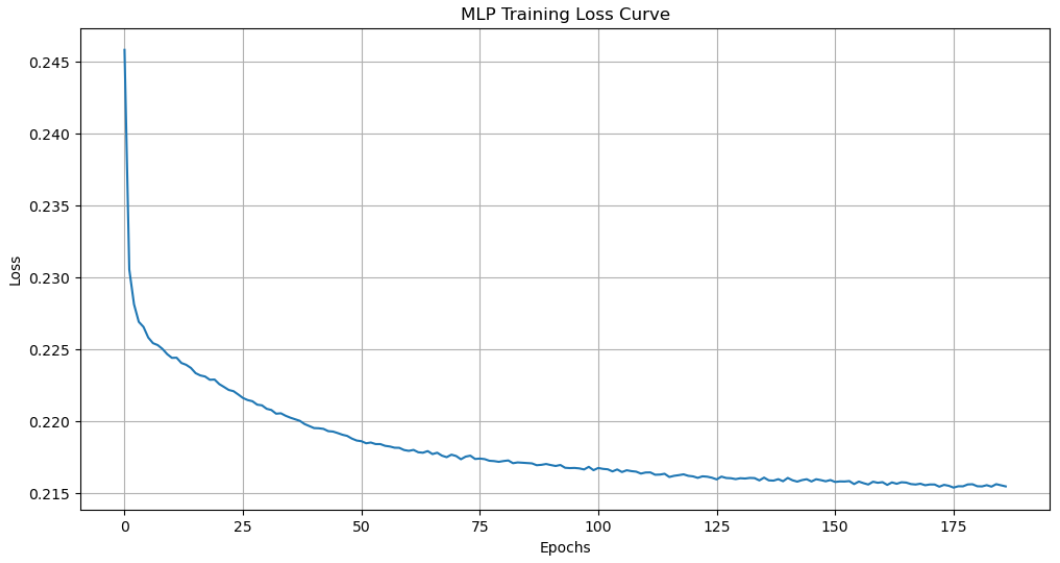
\includegraphics[width=0.9\textwidth]{images/mlp_training_loss.png}
    \caption{\textit{Multi-layer Perceptron}: Curva de perda durante o treino, mostrando a convergência do modelo.}
    \label{fig:mlp_training_loss}
\end{figure}

\begin{figure}[H]
    \centering
    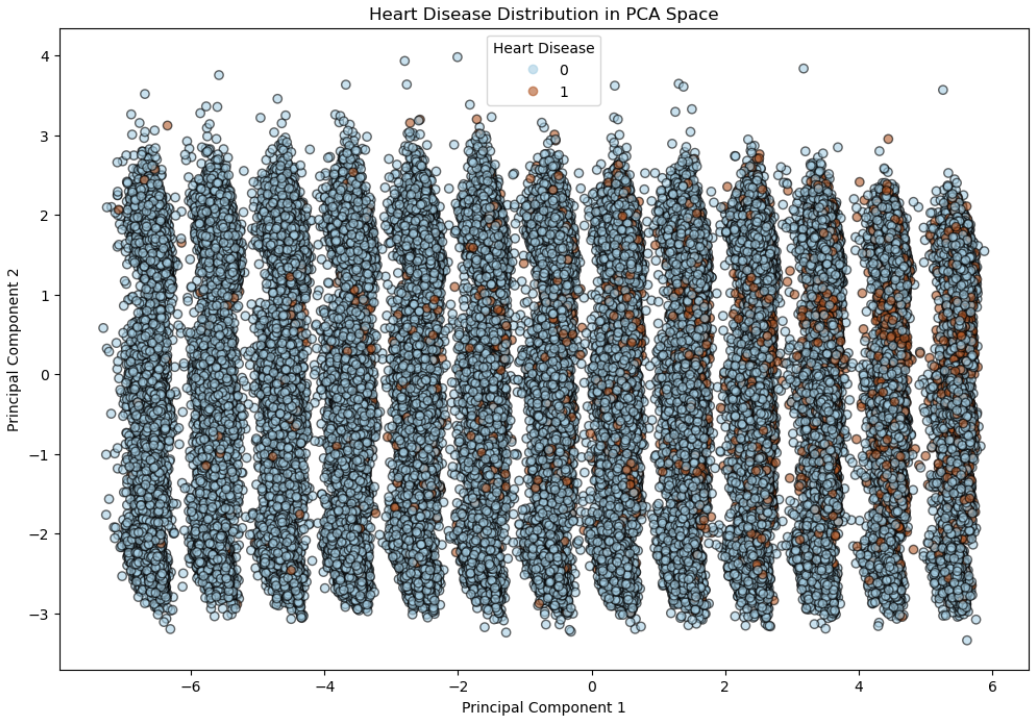
\includegraphics[width=0.9\textwidth]{images/knn_pca.png}
    \caption{\textit{k-NN}: Distribuição dos dados no espaço reduzido para 2 dimensões utilizando \textit{PCA}.}
    \label{fig:knn_pca}
\end{figure}

\section{Métricas individuais de modelos}
\begin{figure}[H]
    \centering
    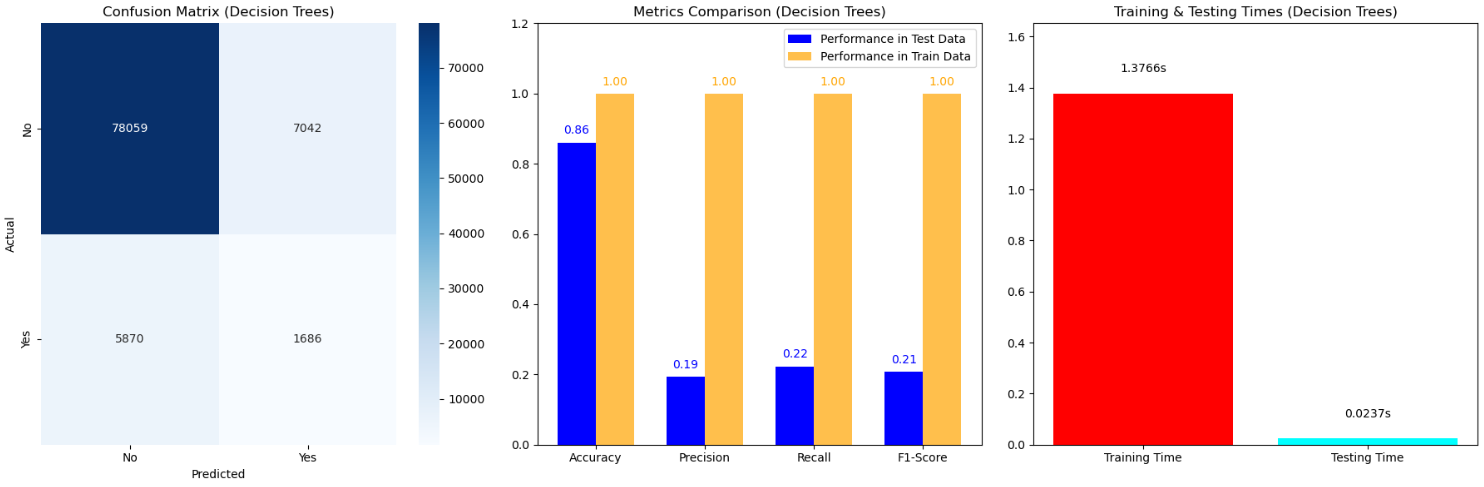
\includegraphics[width=0.9\textwidth]{images/decision_tree_overview.png}
    \caption{Modelo de \textit{Decision Trees}: Matriz de confusão, métricas de desempenho e tempos de execução.}
    \label{fig:decision_tree_overview}
\end{figure}

\begin{figure}[H]
    \centering
    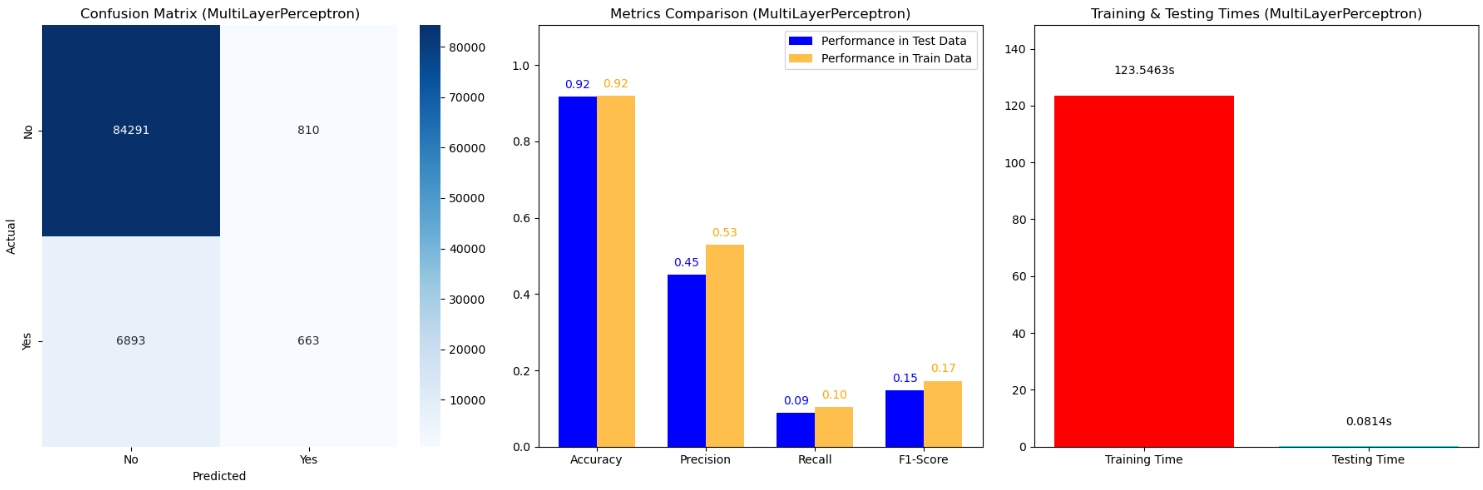
\includegraphics[width=0.9\textwidth]{images/mlp_overview.png}
    \caption{Modelo de \textit{Multi-layer Perceptron}: Matriz de confusão, métricas de desempenho e tempos de execução.}
    \label{fig:mlp_overview}
\end{figure}

\begin{figure}[H]
    \centering
    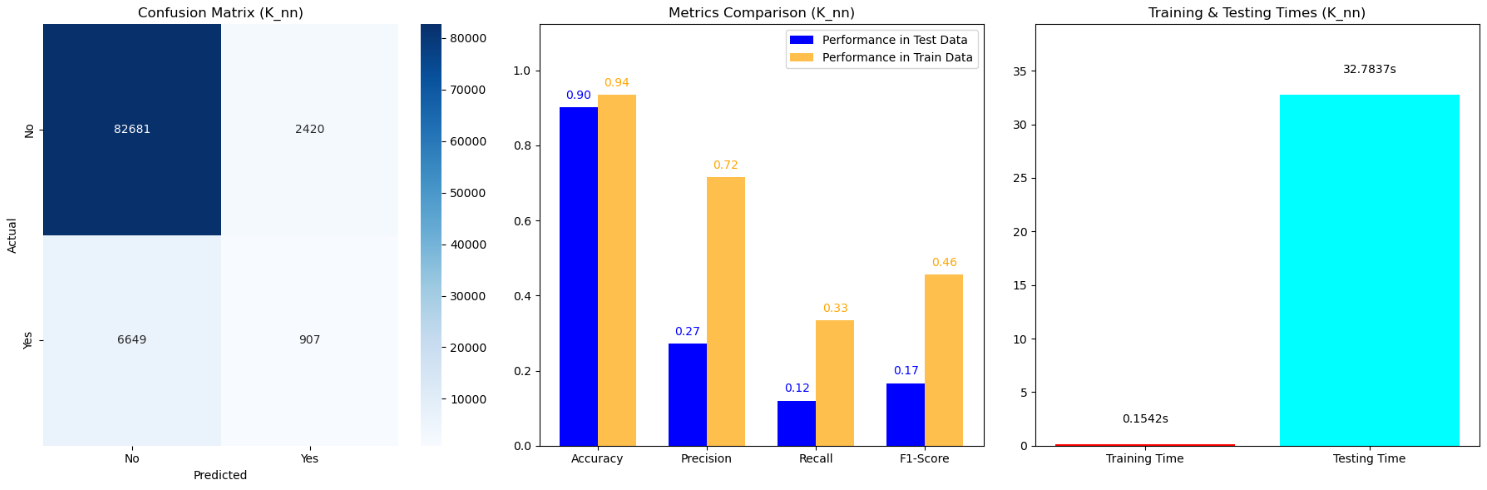
\includegraphics[width=0.9\textwidth]{images/knn_overview.png}
    \caption{Modelo de \textit{k-NN}: Matriz de confusão, métricas de desempenho e tempos de execução.}
    \label{fig:knn_overview}
\end{figure}

\section{Comparações}
\label{chap:comparacoes}

\begin{figure}[H]
    \centering
    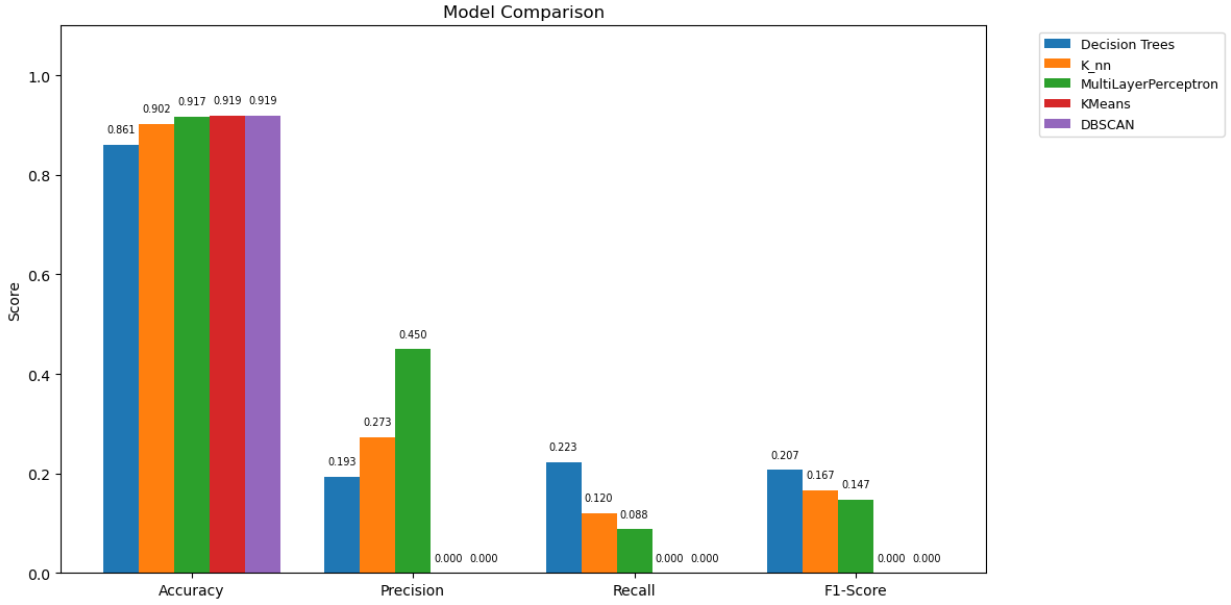
\includegraphics[width=0.9\textwidth]{images/model_comparison.png}
    \caption{Comparação geral do desempenho de todos os modelos.}
    \label{fig:model_comparison}
\end{figure}

\begin{figure}[H]
    \centering
    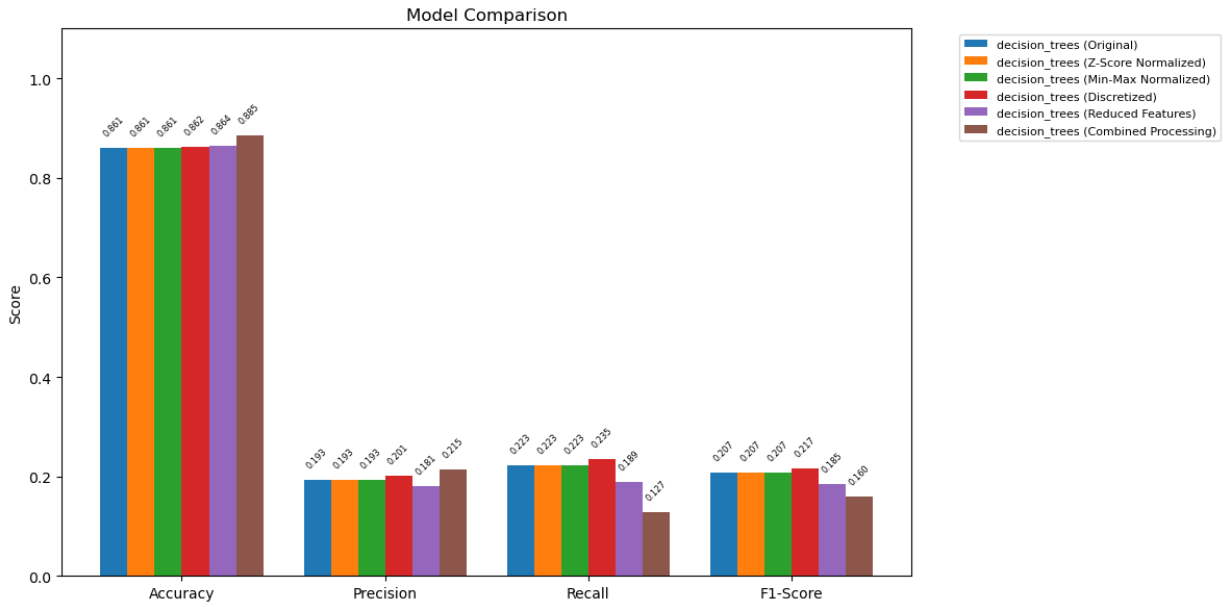
\includegraphics[width=0.9\textwidth]{images/decision_trees_comparison.png}
    \caption{\textit{Decision Trees}: Impacto de diferentes preparações dos dados no desempenho do modelo.}
    \label{fig:decision_trees_comparison}
\end{figure}

\begin{figure}[H]
    \centering
    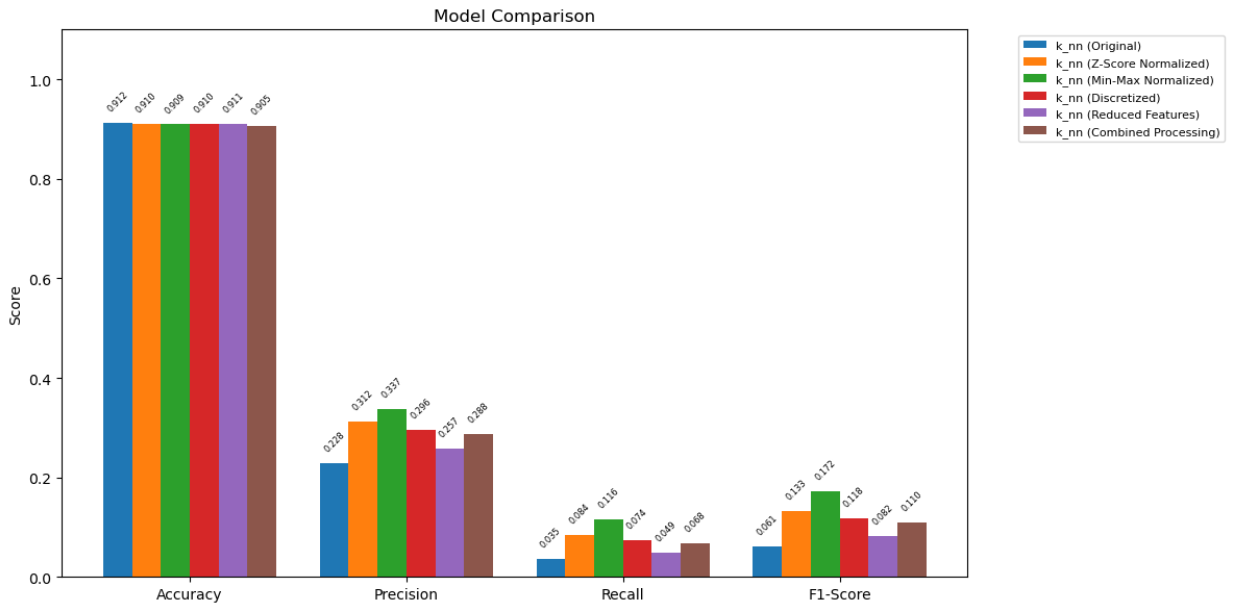
\includegraphics[width=0.9\textwidth]{images/knn_comparison.png}
    \caption{\textit{k-NN}: Impacto de diferentes preparações dos dados no desempenho do modelo.}
    \label{fig:knn_comparison}
\end{figure}

\begin{figure}[H]
    \centering
    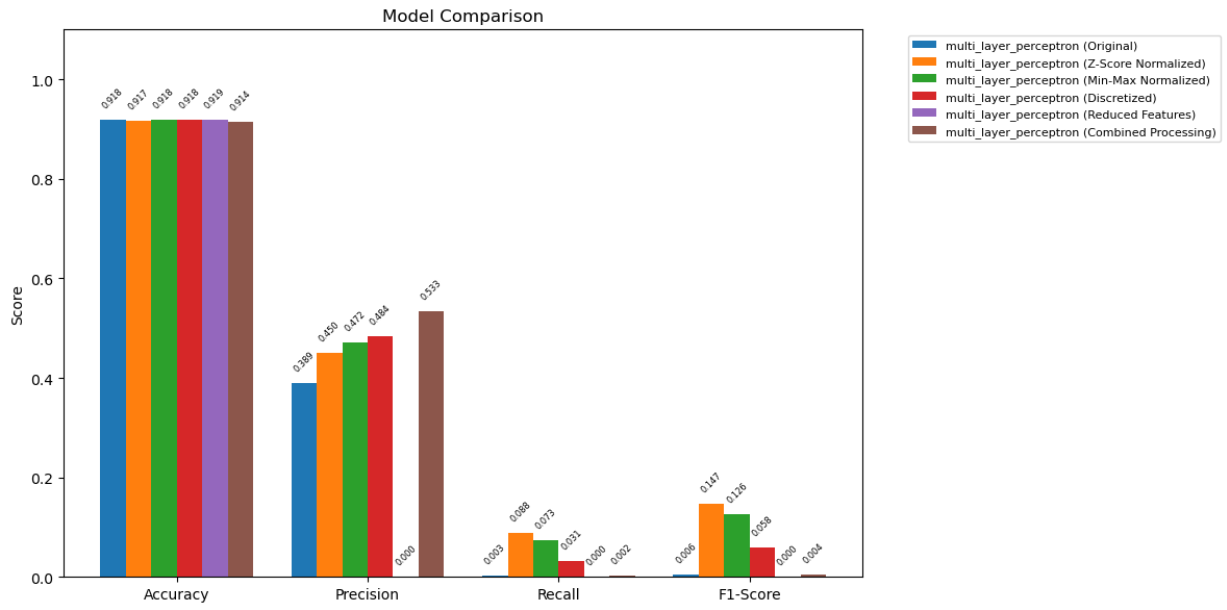
\includegraphics[width=0.9\textwidth]{images/mlp_comparison.png}
    \caption{\textit{Multi-layer Perceptron}: Impacto de diferentes preparações dos dados no desempenho do modelo.}
    \label{fig:mlp_comparison}
\end{figure}



\end{document}